\documentclass[12pt,a4paper,oneside]{report}
\usepackage{fontspec}
\setmainfont{Noto Sans CJK SC}
\setsansfont{Noto Sans CJK SC}
\setmonofont{DejaVu Sans Mono}
\XeTeXlinebreaklocale "zh"
\XeTeXlinebreakskip = 0pt plus 1pt
\usepackage[margin=2.55cm]{geometry}
\usepackage{booktabs,longtable,array,tabularx}
\usepackage{graphicx,xcolor}
\usepackage{amsmath,amssymb}
\usepackage{hyperref}
\usepackage{fancyhdr}
\usepackage{url}
\hypersetup{colorlinks=true,linkcolor=blue!45!black,urlcolor=blue!55!black,
pdftitle={V4-SCOPE-RL：硬安全动作掩码强化学习研究附录},pdfauthor={项目论文技术稿}}
\definecolor{vblue}{HTML}{1769AA}
\definecolor{vgreen}{HTML}{168A72}
\definecolor{vred}{HTML}{C74440}
\definecolor{vgray}{HTML}{667085}
\pagestyle{fancy}
\fancyhf{}
\fancyhead[L]{FAM-TEB / V4-SCOPE-RL 研究附录}
\fancyhead[R]{\leftmark}
\fancyfoot[C]{V4--\thepage}
\setlength{\headheight}{15pt}
\setlength{\parindent}{2em}
\setlength{\parskip}{0.35em}
\newcommand{\ok}{\textcolor{vgreen}{通过}}
\newcommand{\fail}{\textcolor{vred}{失败}}
\newcommand{\scope}{\textcolor{vgray}{证据边界}}
\newcommand{\code}[1]{\texttt{#1}}

\title{\Huge V4-SCOPE-RL\\[0.4em]
\Large 基于硬安全动作掩码的候选轨迹强化学习\\[0.8em]
\large 论文研究附录与终局阴性结果}
\author{项目论文技术稿\\\small 从冻结合同、训练回执与 fresh-seed 证据自动导出}
\date{2026 年 8 月 7 日}

\begin{document}
\special{pdf:trailerid [<5634524C535550504C454D454E543031><5634524C535550504C454D454E543031>]}
\pagenumbering{Roman}
\maketitle

\chapter*{范围声明}
\addcontentsline{toc}{chapter}{范围声明}
本附录在冻结 V3-SCOPE 证据之后建立独立的 V4-SCOPE-RL。V4 没有改写 V2/V3 结果，
没有连接稳定实车工作区，没有发布实车命令，也没有进行在线 TEB 参数写入。研究只使用
确定性快速交互仿真；由于预注册学习门失败，Gazebo、Actual TEB 正式比较和实车阶段均未启动。

本研究的完整结论是：\textbf{强化学习模块与硬安全动作掩码已经实现并通过组件测试，但没有
证明其相对同候选集解析排序器具有有意义的效率提升。} 该阴性结果不是“无结果”；它给出了
动作支持、训练预算、选模规则和学习价值边界，为论文中“何时不应启用强化学习”提供可复核证据。

\chapter*{摘要}
\addcontentsline{toc}{chapter}{摘要}
V3-SCOPE 使用解析函数在经过 Ackermann 可行性与硬安全验证的候选中进行一次性选择。为研究
动态 actor 响应下的序列决策价值，本附录提出 V4-SCOPE-RL：以 0.25 s 周期重复构建候选，
硬验证器产生布尔安全动作掩码，Masked-PPO 只能在掩码允许的候选 ID 上采样和更新。学习器无权
改变候选几何、运动学、占据预测、安全阈值、certified-stop 回退和
\path{/cmd_vel_navigation} 命令边界。

全局预算冻结为三轮单因素、600,000 个训练环境步和 240 个未使用的 Gazebo 单元。初始探针、
响应持续时间因素、时间奖励对齐因素和最终 actor 响应率因素均被完整保存。两个训练种子的最佳
验证改善仅为 0.104\% 和 0.073\%，低于 3\% 学习门。终局 30 个 fresh paired blocks 中，
解析/Masked-PPO 均为 30/30 成功、0 接触、0 掩码违规，受限时间为 7.7750/7.7667 s；配对相对
降幅仅 0.0980\%，双侧 95\% block-bootstrap 区间为 [0, 0.2941\%]，仅 1/30 块为正。
因此不支持显著或有意义的学习优化声明，但支持“模块实现、掩码完整性和失败关闭”的工程结论。

\noindent\textbf{关键词：} 安全强化学习；无效动作掩码；PPO；Ackermann 轨迹；反应式 actor；
预注册阴性结果

\tableofcontents
\listoftables
\listoffigures
\clearpage
\pagenumbering{arabic}

\chapter{研究动机与问题定义}
\section{从 V3 解析排序到 V4 序列决策}
V3 的正式 Gazebo 比较在共同门状态生成一次候选集合，选择一条空间轨迹并跟踪到目标。V3-04
学习审计发现：308/308 次决策都有解析候选可用，183 次决策有多个安全候选，但解析选择的立即
进度后悔为零；同时，日志对未执行动作的 propensity 为零，不支持离线序列强化学习。这说明
直接把一个神经网络叠加在 V3 日志上既无识别基础，也不能形成可信论文贡献。

V4 改变的是\emph{决策过程}而不是安全边界：在反应式 actor 会受早期自车动作影响的环境中，
每 0.25 s 重新决策。研究问题冻结为：在任务成功和硬安全门不退化的前提下，Masked-PPO 是否
能将 failure-inclusive restricted time 相对解析排序器至少降低 3\%？相对 Actual TEB 的结果
只能作为次要问题，且不能替代与解析排序器的直接比较。

\section{预注册假设与停止规则}
阳性判定必须同时满足：目标成功率不劣于解析基线、接触为零、掩码违规为零、激活复核失败为零、
配对时间点估计至少 3\%，并且独立训练种子方向一致。每轮只允许改变一个因素；淘汰预算不可回收，
不允许使用测试结果选检查点、替换不利种子或删除 timeout。三轮结束后，无论结果如何均停止训练。

\chapter{V4-SCOPE-RL 架构}
\section{学习权限与安全权限分离}
\begin{figure}[htbp]
  \centering
  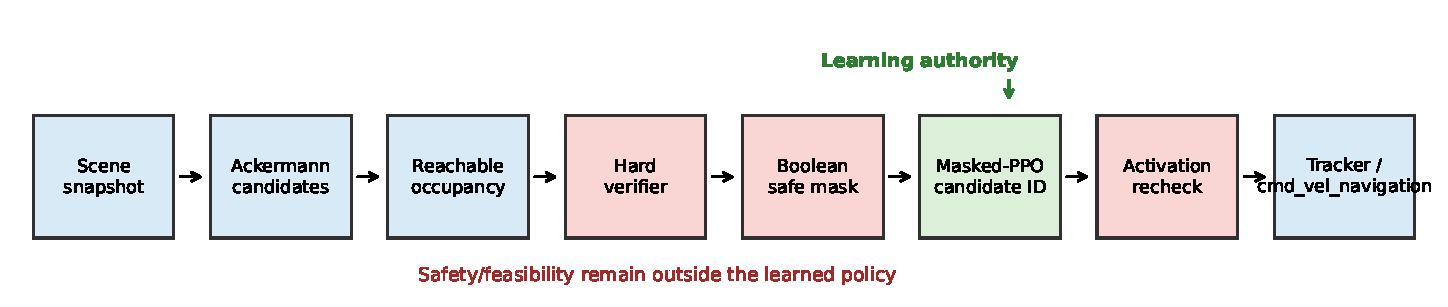
\includegraphics[width=\textwidth]{figure_v4_architecture.pdf}
  \caption{V4-SCOPE-RL 数据流。绿色模块是唯一学习权限；红色模块保持为硬安全边界。}
  \label{fig:v4arch}
\end{figure}

如图~\ref{fig:v4arch}，策略输出是离散候选 ID，不是速度、转角或 TEB 参数。固定动作支持包含
certified stop、0.4/0.8/1.2 m/s 直行候选以及左右空间候选。所有候选先由 Ackermann 运动学生成，
再与 actor 可达占据进行保守距离检查。停止候选始终存在；掩码为空被视为程序错误并失败关闭。

对于策略网络输出的 logits $z_\theta(s,a)$ 和硬验证掩码 $m(s,a)\in\{0,1\}$，实际分布使用
\begin{equation}
\tilde z_\theta(s,a)=
\begin{cases}
z_\theta(s,a),&m(s,a)=1,\\
-\infty,&m(s,a)=0,
\end{cases}
\qquad
\pi_\theta(a\mid s,m)=\operatorname{softmax}(\tilde z_\theta).
\end{equation}
因此被拒绝动作的采样概率和对应 logit 梯度均为零。该设计与无效动作掩码的策略梯度分析一致
\cite{huang2020masking}，在系统角色上接近 pre-shielding：安全层先给出允许动作集合，再由学习器
选择\cite{alshiekh2018shielding}。不过，本项目仅验证实现与经验门，不声称形式化安全。

\section{状态、奖励与 Masked-PPO}
状态由 12 个全局特征和 $6\times5$ 个候选特征组成：自车进度、横向位置、航向、速度、前一动作，
actor 坐标、速度与加速度估计、到达时间差，以及每个候选的接受位、投影进度、保守净空、加速度
代价和横向偏移。网络为两层 128 单元 Tanh actor--critic。PPO 使用裁剪代理目标
\begin{equation}
L^{\mathrm{clip}}(\theta)=\mathbb{E}_t\left[
\min\left(r_t(\theta)\hat A_t,
\operatorname{clip}(r_t(\theta),1-\epsilon,1+\epsilon)\hat A_t\right)\right],
\end{equation}
其中概率比 $r_t$ 在同一个硬掩码分布上计算\cite{schulman2017ppo}。安全不是可交换的碰撞惩罚；
奖励只在安全集合内优化进度、耗时、速度变化、动作切换、目标和 timeout。

\chapter{实验合同与实现验证}
\section{预算和身份隔离}
表~\ref{tab:stages} 列出完整闭合链。R0 使用 100,000 步；F1 为 150,000 步；F2 的两个种子各
150,000 步；F3 使用最后 50,000 步，总计恰好 600,000 步。每个阶段使用不同的审计、验证或
终局 fresh seed 区间。测试种子不参与任何拟合和选模。

\begin{table}[htbp]
\centering
\caption{V4 单因素阶段与冻结判定}
\label{tab:stages}
\begin{tabularx}{\textwidth}{p{2.5cm}Xrrp{2.2cm}}
\toprule
阶段 & 唯一变化/目的 & 训练步 & 最佳改善 & 结论\\
\midrule
V4-02-R0 & 基线开发探针 & 100,000 & 0.000\% & \fail\\
V4-03-F1 & actor 让行响应持续时间 & 150,000 & 0.000\% & \fail\\
V4-03-F2/4103 & 耗时奖励与主指标对齐 & 150,000 & 0.104\% & \fail\\
V4-03-F2/4104 & 独立训练种子复核 & 150,000 & 0.073\% & \fail\\
V4-03-F3 & actor 纵向响应率 & 50,000 & 0.000\% & \fail\\
V4-04-N1 & 30 个 fresh 终局刻画 & 0 & 0.098\% & 阴性闭合\\
\bottomrule
\end{tabularx}
\end{table}

\section{学习价值与组件门}
F1 在训练前执行 100 个新状态块、600 个候选反事实回合。安全多动作状态比例为 100\%，17\% 的
块存在正序列后悔，超过 5\% 启动门；但平均后悔仅 0.6165\%，已经提示可学习效应很小。F3 在训练
前又运行 1000 个均匀随机安全掩码回合，得到 0 接触、0 掩码违规和最小经验净空 0.3172 m。
最终 Python 测试共 9 项，覆盖合同、停止候选、拒绝动作不投影、克隆重放、掩码概率、短训练和
检查点往返，9/9 通过。

\chapter{结果}
\section{训练与验证结果}
\begin{figure}[htbp]
  \centering
  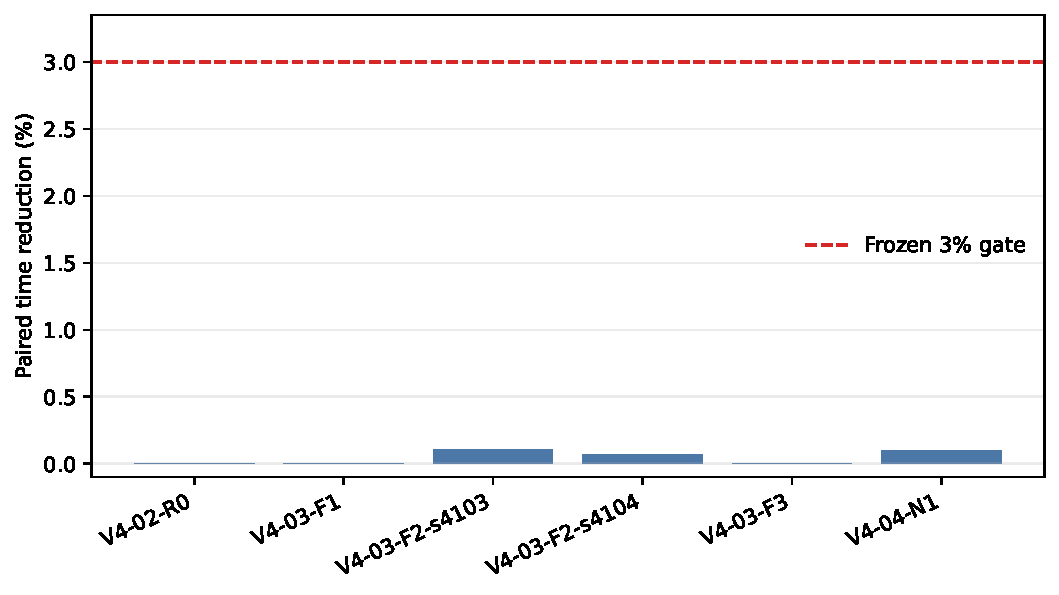
\includegraphics[width=0.88\textwidth]{figure_v4_factor_history.pdf}
  \caption{三轮单因素与终局刻画的配对时间降幅。虚线为冻结的 3\% 门。}
  \label{fig:factor}
\end{figure}

图~\ref{fig:factor} 显示 F1 的策略与解析排序器完全相同。F2 提高耗时权重后，两个训练种子都出现
正方向，但只有 0.104\% 和 0.073\%；跨种子均值 0.0883\%。F3 的响应率因素通过随机安全预检，
但策略再次收敛到解析选择。三轮均未接近 3\% 门，继续增加预算没有预注册依据。

\section{Fresh-seed 终局刻画}
冻结 F2 中验证回报最高的 seed4104 检查点后，V4-04-N1 使用 seeds 430100--430129 运行 30 个
新配对块。表~\ref{tab:fresh} 汇总结果。

\begin{table}[htbp]
\centering
\caption{V4-04-N1 fresh-seed 快速仿真结果}
\label{tab:fresh}
\begin{tabular}{lrrrr}
\toprule
方法 & 成功 & 受限均时/s & 接触 & 掩码违规\\
\midrule
同候选集递推解析排序 & 30/30 & 7.7750 & 0 & 0\\
Masked-PPO seed4104 & 30/30 & 7.7667 & 0 & 0\\
\bottomrule
\end{tabular}
\end{table}

配对相对降幅为 0.0980\%，双侧 95\% paired-block percentile bootstrap 区间为
$[0,0.2941\%]$。只有一个块缩短 0.25 s，其余 29 个块完全相同（图~\ref{fig:paired}）。因此区间
没有显示负方向并不等于存在实质收益：点估计只有冻结最小效应 3\% 的约 1/31。

\begin{figure}[htbp]
  \centering
  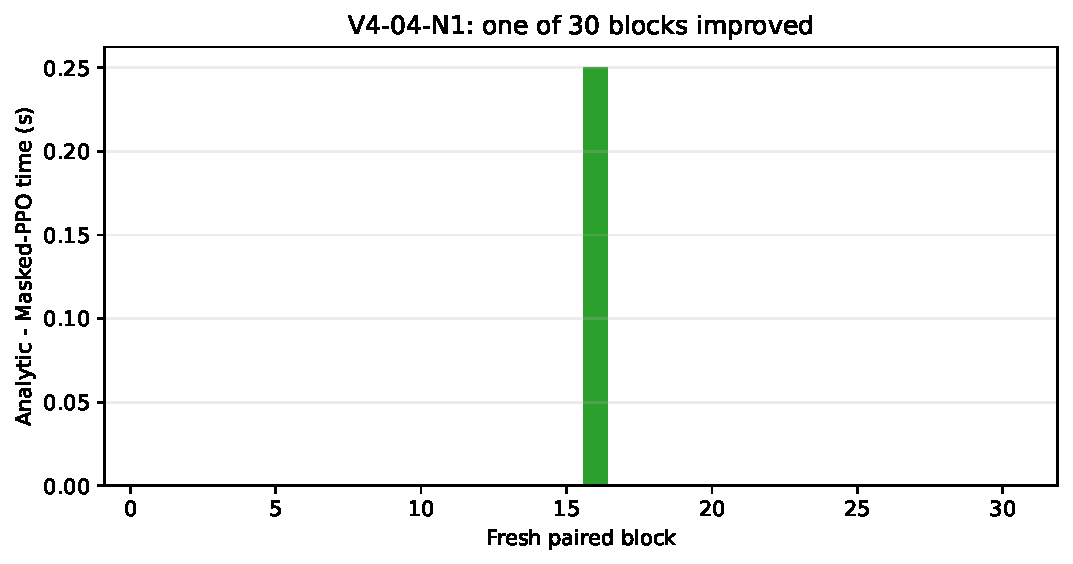
\includegraphics[width=0.88\textwidth]{figure_v4_fresh_paired_differences.pdf}
  \caption{每个 fresh block 的解析时间减 Masked-PPO 时间。29/30 为零。}
  \label{fig:paired}
\end{figure}

\begin{figure}[htbp]
  \centering
  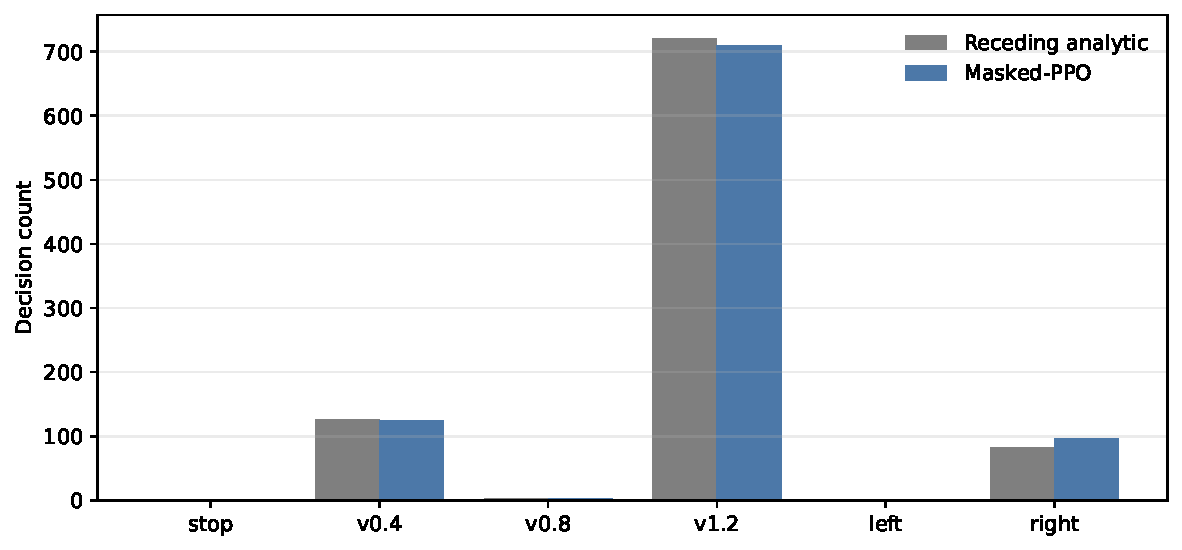
\includegraphics[width=0.88\textwidth]{figure_v4_action_distribution.pdf}
  \caption{30 个 fresh blocks 中两种方法的动作计数。学习策略整体复现解析决策。}
  \label{fig:actions}
\end{figure}

\chapter{讨论与论文结论}
\section{为什么强化学习没有产生有意义的增益}
结果并非 PPO 数值发散：所有种子安全和任务门稳定，回报收敛且检查点可重放。主要限制是
\textbf{安全候选集合中的长程后悔太小}。解析排序器已经在每个 0.25 s 周期重算安全集并优先选择
投影进度最大的动作；绝大多数块中，长期最优动作与立即解析动作一致。F1 的反事实审计虽然通过
“存在性”门，但平均可利用后悔只有 0.62\%。这不足以支撑 3\% 的论文效应，更不应通过增加网络
规模、替换种子或放宽门槛来制造阳性。

\section{可以写入论文的贡献}
第一，V4 提供了一个真实可运行的 RL 模块，而不是把 V3 解析器改名为学习器：包含 Gymnasium
序列环境、Masked-PPO actor--critic、GAE、裁剪更新、多环境 rollout、检查点和确定性评测。
第二，学习权限与安全权限严格分离；1000 个随机掩码预检和 30 个 fresh 配对块均为 0 接触、0
掩码违规。第三，预注册三轮因素给出了重要阴性认识：在安全候选已经由强解析器近似饱和时，
“加入 RL”本身不是性能贡献。第四，所有不利结果、超参数、种子和停止条件被保留，可作为论文的
消融、局限性和研究诚信材料。

\section{不能写入论文的声明}
本研究没有 V4 Gazebo 结果，不能声称 V4 优于 Actual TEB；没有多人、感知、OOD 或真实硬件结果；
经验上的 0 接触不是形式化安全证明；0.098\% 点改善也不是显著或有意义的强化学习收益。
历史 V3-11 的 scoped Gazebo 阳性和 V3-21 的失效计入式阴性仍应分别报告，不能与 V4 快速仿真
合并成一个更有利的总体效应。

\section{后续研究建议}
若未来重新开启新研究，不应继续当前超参数搜索。合理入口是先引入具有可识别长程后悔的新任务
族，例如多 actor 次序协商、遮挡下的信息收集动作或明确的机会成本，再以独立几何和 fresh seed
重新做学习价值审计。只有同候选集解析控制上存在足够的序列 regret，强化学习比较才有统计功效。
任何 Gazebo 或实车阶段都需要新的合同、预算和授权。

\chapter{复现资源索引}
机器可读资源位于 \path{artifacts/v4/paper/v4_06_p1_thesis_export/}：
\begin{itemize}
  \item \path{v4_04_n1_method_summary.csv}：方法级主表；
  \item \path{v4_04_n1_paired_blocks.csv}：30 个配对块；
  \item \path{v4_factor_history.csv}：全部训练因素与预算；
  \item \path{v4_06_p1_claims.yaml}：允许与禁止声明；
  \item 三幅 SVG/PDF 结果图和一幅架构图；
  \item \path{v4_06_p1_evidence_manifest.sha256}：路径--SHA256 证据清单。
\end{itemize}
核心实现位于 \path{src/application/v4_scope_rl/}。组件测试 XML 为
\path{artifacts/v4/v4_component_tests.xml}。历史 V3 论文 PDF 保持原 SHA，不被覆盖；最终合并稿只在
其后追加本附录。

\begin{thebibliography}{9}
\bibitem{schulman2017ppo}
J. Schulman, F. Wolski, P. Dhariwal, A. Radford, and O. Klimov,
``Proximal Policy Optimization Algorithms,'' arXiv:1707.06347, 2017.
\url{https://arxiv.org/abs/1707.06347}

\bibitem{huang2020masking}
S. Huang and S. Ontañón,
``A Closer Look at Invalid Action Masking in Policy Gradient Algorithms,''
arXiv:2006.14171, 2020.
\url{https://arxiv.org/abs/2006.14171}

\bibitem{alshiekh2018shielding}
M. Alshiekh et al., ``Safe Reinforcement Learning via Shielding,''
Proceedings of the AAAI Conference on Artificial Intelligence, 2018.
\url{https://ojs.aaai.org/index.php/AAAI/article/view/11797}
\end{thebibliography}

\end{document}
